\documentclass{lug}

\usepackage{etoolbox}
\usepackage{etoolbox}
\usepackage{textcomp}
\usepackage[nodisplayskipstretch]{setspace}
\usepackage{xspace}
\usepackage{enumitem}

\setitemize{label=\usebeamerfont*{itemize item}%
  \usebeamercolor[fg]{itemize item}
  \usebeamertemplate{itemize item}}

\AtBeginEnvironment{minted}{\singlespacing\fontsize{10}{10}\selectfont}

\makeatletter
\patchcmd{\beamer@sectionintoc}{\vskip1.5em}{\vskip0.5em}{}{}
\makeatother

\newcommand{\pmidg}[1]{\parbox{\widthof{#1}}{#1}}
\newcommand{\splitslide}[4]{%
    \noindent
    \begin{minipage}{#1 \textwidth - #2 }
        #3
    \end{minipage}%
    \hspace{ \dimexpr #2 * 2 \relax }%
    \begin{minipage}{\textwidth - #1 \textwidth - #2 }
        #4
    \end{minipage}
}
\setbeamerfont{footnote}{size=\tiny}

\title{Universal Packages}
\author{Sumner Evans and Robby Zampino}
\institute{Mines Linux Users Group}

\begin{document}

\section{Introduction}

\begin{frame}{What are packages?}
    \begin{center}
        A \textbf{package} is an archive containing a collection of executable
        files or source code, along with metadata, which represent a computer
        program.
    \end{center}
\end{frame}

\begin{frame}{What is a package format?}
    \begin{center}
        A \textbf{package format} is an organizational structure for delivering
        packages to users.
    \end{center}
\end{frame}

\begin{frame}{Why do we need package formats?}
    \begin{itemize}
        \item They provide a common way to bundle executables, libraries,
            assets, etc.\ for deployment on user machines.
        \item They provide metadata about programs for use in package managers.
        \item It would suck if we had to go find the source code for every
            single program we want to use and compile from
            source.\footnote[frame]{Actually, some package formats do require
            compilation from source (for example some AUR packages) but at least
            it helps automate this process.}
    \end{itemize}
\end{frame}

\begin{frame}{A bit of history}
    \begin{enumerate}[leftmargin=2cm]
        \item[1994] \texttt{dpkg} --- the package format behind \texttt{apt} and
            \texttt{apt-get}.  Used by Debian-based systems.
        \item[1997] \texttt{RPM} --- the package format behind \texttt{yum} and
            \texttt{dnf}. Used by RHEL-like systems.
        \item[2002] \texttt{pacman} --- the package manager for Arch Linux. It
            just uses \texttt{tar} files.
        \item[2004] \texttt{klik}/\texttt{PortableLinuxApps}
            (2011)/\texttt{AppImage} (2013) --- a package format built to be
            Linux-distro agnostic.
        \item[2006] \texttt{nix} --- a purely functional package format.
            Primarily used by NixOS.
        \item[June 2016] \texttt{snapd} --- the Canonical-backed universal
            package format is ported to a wide range of Linux distros.
        \item[June 2016] \texttt{Flatpak} --- the Red Hat-backed universal
            package format becomes generally available.
    \end{enumerate}
\end{frame}

\section{Universal Package Formats}
\begin{frame}{Common objectives}
    \begin{itemize}
        \item Linux distro agnosticism
        \item Solve the ``dependency hell''
        \item Create a ``single'' deployment target for all of Linux
    \end{itemize}
\end{frame}

\section{AppImage}
\begin{frame}{Why is AppImage cool?}
    \begin{itemize}
        \item \textbf{AppImage does not require installation.} The AppImage file
            is just its compressed image that is mounted with FUSE when it runs.
        \item \textbf{AppImage does not require root permission.} The
            application is run as the user and the base system is left
            untouched.
        \item \textbf{The AppImage itself is executable.} Just \texttt{chmod +x}
            the \texttt{.AppImage} file and run.
        \item \textbf{Linus says so}
            \begin{quote}
                ``This is just very cool.''\\
                \hspace*{0.5in}\textasciitilde\ Linus Torvalds
            \end{quote}
    \end{itemize}
\end{frame}

\begin{frame}{How does AppImage work?}
    Application developers use the \texttt{appimagetool} converts an AppDir into
    a self-mounting filesystem image.

    AppImages can be integrated with the system via menu entries, icons, MIME
    types, etc. The \texttt{appimaged} daemon handles this registering and
    unregistering process.
\end{frame}

\begin{frame}{How to create an AppImage}
    Create an AppDir with the following files (totally copied from their
    documentation):
    \begin{itemize}
        \item The files of the original application.
        \item A \texttt{.desktop} file that tells \texttt{appimagetool}
            about the name of the application, and the icon it should
            use.
        \item A PNG, SVG or an XPM icon with the name given in the
            \texttt{.desktop} file with the Icon entry.
        \item An AppRun file, which is used to start up the application
            inside the filesystem. Once the AppImage ELF has mounted the
            filesystem, it invokes this file. In the AppRun file, you
            can run some initialization procedures (such as setting
            environment variables), and then start up the real
            application.
        \item Optionally, you should also add AppStream metadata in
            \texttt{usr/share/metainfo}.
    \end{itemize}
\end{frame}

\begin{frame}
    \Huge
    Live Demo: Running an AppImage
\end{frame}

\section{Snaps \& \texttt{snapd}}
\begin{frame}{Why are Snaps cool?}
    \begin{itemize}
        \item \textbf{Snaps are \texttt{squashFS} filesystems.} They contain
            your app code and a \texttt{snap.yaml} file with metadata.
        \item \textbf{Snaps are self-contained.} The necessary libraries and
            runtimes are bundled in the snap. This allows you to have different
            library versions in your application than exist on your base system.
        \item \textbf{Snaps can have different levels confinement.}
            \begin{itemize}
                \small
                \item \texttt{strict} is the default policy. The snap has read
                    and/or write rights only in its own install space and
                    selected areas.
                \item \texttt{devmode} is for development of Snaps.
                \item \texttt{classic} confinement behaves as a traditionally
                    packaged application, with full access to the system.
            \end{itemize}
        \item \textbf{Snaps can communicate with one another via
            \textit{interfaces}.}
    \end{itemize}
\end{frame}

\begin{frame}{How do Snaps work?}
    \center
    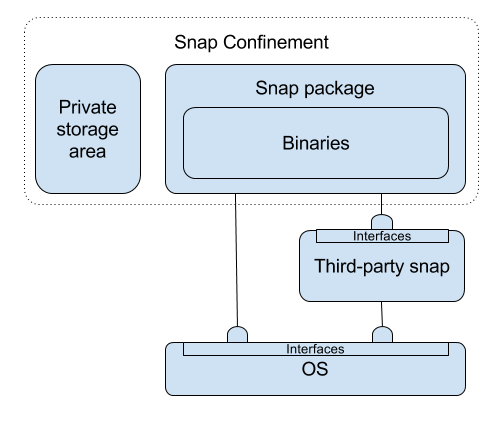
\includegraphics[width=0.9\textwidth]{./graphics/snap_arch}
\end{frame}

\begin{frame}{How to create a Snap}
    \begin{itemize}
        \item Make your application.
        \item Make a \texttt{snapcraft.yaml} with a bunch of stuff.
            \begin{itemize}
                \item name
                \item version
                \item summary
                \item description
                \item grade
                \item confinement
                \item \dots
            \end{itemize}
        \item Run \texttt{snapcraft}.
    \end{itemize}
\end{frame}

\begin{frame}
    \Huge
    Live Demo: Running a Snap
\end{frame}

\section{flatpak}
\begin{frame}{flatpak}
    \begin{itemize}
        \item Flatpak is a system for building, distributing and running sandboxed desktop applications on Linux. (https://github.com/flatpak/flatpak)
    \end{itemize}
\end{frame}

\begin{frame}{Why is flatpak cool?}
    \begin{itemize}
        \item Flatpak includes a system of runtimes that allow developers to build their application against a stable base.
        \item Runtimes allow dedeuplication of dependencies between packages
        \item Flatpak makes uses of bubblewrap for sandboxing
        \item Flatpak supports a system of Appstream metadata to allow packages to show up nicely in various package managers
    \end{itemize}
\end{frame}

\begin{frame}{flatpak Overview}
    \center
    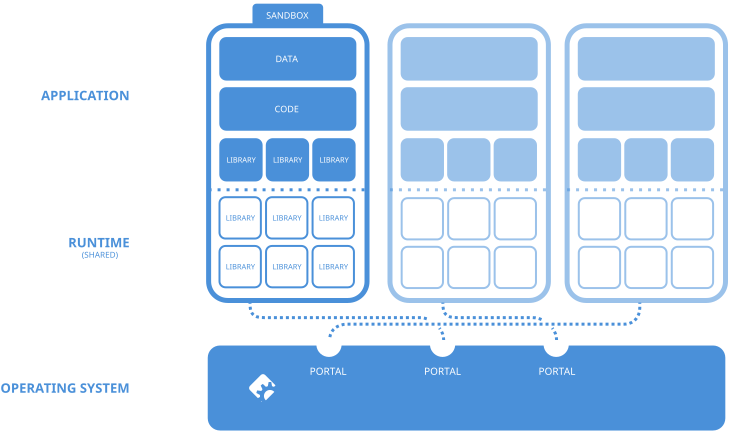
\includegraphics[width=0.9\textwidth]{./graphics/flatpak_overview.png}
\end{frame}

\begin{frame}{Runtimes}
    \begin{itemize}
        \item org.freedesktop.Platform
            \begin{itemize}
                \item D-Bus
                \item GLib
                \item PulseAudio
                \item X11
                \item Wayland
            \end{itemize}
        \item org.gnome.Platform (based on freedesktop)
            \begin{itemize}
                \item GStreamer
                \item PyGObject
                \item Vala
                \item GVFS
                \item other stuff to make Gnome work...
            \end{itemize}
    \end{itemize}
\end{frame}

\begin{frame}{Runtimes}
    \begin{itemize}
        \item org.kde.Platform
            \begin{itemize}
                \item Qt Frameworks
                \item KDE Frameworks
            \end{itemize}
    \end{itemize}
\end{frame}

\begin{frame}{Sandboxing}
    \begin{itemize}
        \item All processes run as the user with no capabilities
        \item All processes run in a transient systemd user scope with the name \texttt{flatpak-\$appid-\$pid}
        \item \texttt{/} is a private tmpfs not visible anywhere else. This is \texttt{pivot\_root:ed} into so it is the new  and all other mounts from the host are unmounted from the namespace.
        \item Enviroment variables set:
        \begin{itemize}
            \item {PATH=/app/bin:/usr/bin}
            \item {LD\_LIBRARY\_PATH=/app/lib}
            \item {XDG\_CONFIG\_DIRS=/app/etc/xdg:/etc/xdg}
            \item {XDG\_DATA\_DIRS=/app/share:/usr/share}
            \item {XDG\_RUNTIME\_DIR=/run/user/\$pid}
        \end{itemize}    
    \end{itemize}
\end{frame}


\section{How to build a flatpak package}

\begin{frame}{flatpak-builder}
    \begin{itemize}
        \item Install the flatpak-builder package
        \item See https://flatpak.org/getting.html for instructions
    \end{itemize}
\end{frame}

\begin{frame}{Runtimes}
    \begin{itemize}
        \item Add the respository hosting your runtime 
        \item\texttt{\$\ flatpak remote-add --if-not-exists flathub https://flathub.org/repo/flathub.flatpakrepo}
        \item Install the runtime and corresponding SDK
        \item\texttt{\$\ flatpak install flathub org.freedesktop.Platform//1.6 org.freedesktop.Sdk//1.6}
    \end{itemize}
\end{frame}

\begin{frame}{Manifest}
    \center
    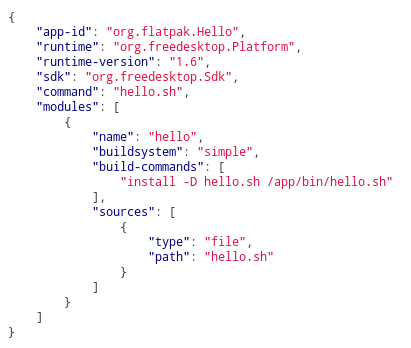
\includegraphics[width=0.9\textwidth]{./graphics/flatpak_json.png}
\end{frame}

\begin{frame}{Packagin}
    \begin{itemize}
        \item \texttt{\$\ flatpak-builder app-dir org.flatpak.Hello.json}
        \item \texttt{\$\ flatpak-builder --run app-dir org.flatpak.Hello.json hello.sh}
    \end{itemize}
\end{frame}


\section{nix}

\section{Comparison}
\begin{frame}{Advantages of each of these universal package formats}
    \begin{itemize}
        \item AppImage is great for portable, self-contained applications.
        \item Snaps are good for deploying single applications.
        \item Flatpak is good for distributing a set of applications. For
            example Gnome development builds are in a Flatpak repository.
    \end{itemize}
\end{frame}

\section{Love to Hate Them}

\begin{frame}{Proprietary enterprise applications are coming to Linux}
    Currently, when enterprises want to make a cross-platform application, they
    see this:
    \begin{enumerate}[leftmargin=2cm]
        \item[macOS] \texttt{.dmg}
        \item[Windows] \texttt{.exe}
        \item[Linux] \texttt{.deb} and \texttt{.rpm} and \texttt{PKGBUILD} and
            \dots, then deal with the dependency hell\footnote[frame]{Yes, you
            have to deal with dependency hell on other platforms too, but every
            platform has a different type of dependency hell. Coming to Linux is
            an expensive prospect for many enterprises.}
    \end{enumerate}

    However, when companies like Canonical come in and say ``just target
    snaps'', all of a sudden, it may tip the scale at enterprises for them to
    start targeting Linux. If they create a snap, then they capture all of the
    Linux market, not just the subset that uses a particular format.
\end{frame}

\begin{frame}{Pros and cons}
    \textbf{Pros}
    \begin{itemize}
        \item More application availability.
        \item More abstraction! No more dealing with a bunch of different
            packaging formats.
    \end{itemize}

    \textbf{Cons}
    \begin{itemize}
        \item The applications are going to be crap. Bloated, Electron,
            enterprise crap.
        \item More abstraction! Not much improvement on ease of deployment in
            comparison to deploying to \texttt{.deb}.
    \end{itemize}
\end{frame}

% TODO: if time
% \begin{frame}
%     \Huge
%     Live Demo: Packaging Something
% \end{frame}

\begin{frame}[standout]
    \Huge
    Questions?
\end{frame}

\begin{frame}{Resources}
    \begin{enumerate}[leftmargin=2cm]
        \item[AppImage] \url{https://appimage.org/}
        \item[Snapcraft] \url{https://snapcraft.io/}
        \item[Flatpak] \url{https://flatpak.org/}
        \item[Nix] \url{https://nixos.org/nix/}
    \end{enumerate}
\end{frame}

\end{document}
